\section{Theory}
\subsection{Majorana Fermion}
{\color{red}
Quick introduction to Majorana fermions, their properties. Discuss the concept of Majorana zero modes (MZMs) and their significance in topological quantum computing.
}
\subsection{Topological Quantum Computing}
{\color{red}
Introduce the concept of topological quantum computing, emphasizing the role of MZMs in encoding and manipulating quantum information. Discuss the advantages of topological quantum computing, such as robustness against local perturbations and decoherence.
}

\subsection{The Superconducting State}
\subsubsection{From Cooper Pairing to the Energy Gap}
Superconductivity arises when electrons in a metal form bound pairs, known as Cooper pairs, below a critical temperature $T_c$. These pairs condense into a coherent quantum state that can carry current without resistance, and also expel magnetic fields via the Meissner effect. This immediately distinguishes a superconductor from a perfect conductor, because it is a distinct thermodynamic phase with long-range quantum coherence \cite{Cambridge_MBPhysics}.\\
The microscopic origin of superconductivity lies in an effective attractive interaction between electrons, mediated by phonons (lattice vibrations). It is somewhat counterintuitive that electrons, which naturally repel each other due to their negative charge, can experience an effective attraction. However, when an electron moves through a lattice structure of positive ions, it distorts the lattice, pulling a group of the ions towards itself. This distortion creates a region of increased positive charge density that can attract another electron with opposite momentum and spin, leading to the formation of a Cooper pair \cite{Physics_libretexts_2025}.\\
Even a weak attraction can destabilize the normal metallic Fermi sea, allowing electrons of opposite momenta and spins to form bound pairs. These pairs behave as bosons (integer spin particles) and condense into a macroscopic quantum state described by a collective wavefunction $ψ(r)$, whose phase coherence gives rise to the supercurrent.\\
At the mean-field level, this collective behaviour opens an energy gap $Δ$ around the Fermi surface. This gap represents the minimum energy needed to break a Cooper pair and create excitations, called Bogoliubov quasiparticles, that are mixtures of electron and hole states. The presence of this gap explains the vanishing resistivity and the exponential suppression of heat capacity and other thermodynamic quantities at low temperatures \cite{Cambridge_MBPhysics}, \cite{BCS}.\\
The pairing gap is what makes superconductors so special for topological applications. Because single-particle excitations cost a finite energy, the superconducting condensate is robust against small perturbations and other local noise. When combined with spin-orbit coupling and appropriate confinement or hybridization, this same pairing mechanism can give rise to topological superconductivity, where the quasiparticles at zero energy behave as Majorana modes.\\
In essence, superconductivity provides both the microscopic pairing mechanism and the macroscopic phase coherence needed to host non-local, topologically protected excitations, making it the natural foundation for exploring Majorana physics in condensed matter systems.

\subsubsection{Bogoliubov-de Gennes Formalism}
While the BCS theory captures the essence of superconductivity as a condensate of Cooper pairs, it assumes a spatially uniform order parameter $Δ$. In real systems, superconductivity can vary across space due to interfaces, impurities, or confinement. To describe such spatially inhomogeneous superconductors, the BCS framework must be generalized. This leads to the Bogoliubov-de Gennes (BdG) formalism \cite{Cambridge_MBPhysics}, \cite{BCS}.\\
\begin{equation}
  \begin{pmatrix}
  H_0(r) & Δ(r) \\
  Δ^{*}(r) & -H_0^{*}(r)
  \end{pmatrix}
  \begin{pmatrix}
  u_n(r) \\
  v_n(r)
  \end{pmatrix}= E_n
  \begin{pmatrix}
  u_n(r) \\
  v_n(r)
  \end{pmatrix}
  \label{eq:BdGintro}
\end{equation}
where $H_0 = \frac{p²}{2m}-μ + V(r)$ describes the normal-state single particle Hamiltonian, and $Δ(r)$ is the superconducting pair potential.\\ 
Each solution of the BdG equations (\ref{eq:BdGintro}) corresponds to a Bogoliubov quasiparticle, a coherent superposition of electron and hole amplitudes $(u_n(r), v_n(r))$. The resulting excitation spectrum is symmetric about zero energy due to the intrinsic particle-hole symmetry of the BdG Hamiltonian:
\begin{equation}
  Ξ H_{BdG} Ξ^{-1} = -H_{BdG}, \quad Ξ = τ_x K
\end{equation}
where $τ_x$ acts in particle-hole space and $K$ is complex conjugation. This ensures that if $E_n$ is an eigenvalue, so is $-E_n$.\\
This symmetry has an important consequence: superconductors no longer conserve particle number, only fermion parity, and the eigenstate at $± E_n$ correspond to the same physical excitation. A zero-energy solution ($E_n = 0$) indicates a self-conjugate quasiparticle, $γ = γ^{†}$, which is the defining property of a Majorana mode \cite{Topocondmat}.\\
The BdG formalism connects the microscopic BCS theory and the modern description of topological superconductivity. It provides a natural framework for modeling hybrid nanostructures, such as quantum dots coupled to superconducting leads, and low-dimensional systems where topological phases can emerge.  \\

\subsubsection{Hybrid Semiconductor-Supercondcutor Systems}
Superconductivity on its own already provides a platform for charge transport without resistance, and for pairing electrons into coherent states. However, when a conventional superconductor is coupled to another material, such as a semiconductor, it can transfer its essential properties through what is known as the \textit{proximity effect}. This hybridization allows us to engineer superconductivity in systems that do not exhibit it intrinsically, and forms an experimental foundation for realizing Majorana modes in condensed matter systems  \cite{Qtech}.
\paragraph{(i) Hybdird Systems:  The Proximity Effect and Induced Superconductivity}
At the interface between a semiconductor and a superconductor, the superconducting condensate can penetrate into the semiconductor, through a process called the proximity effect. As a result, electrons in the semiconductor acquire pairing correlations from the superconductor, giving rise to an induced superconducting gap $Δ_{\mathrm{ind}}$, even though the semiconductor itself lacks an intrinsic pairing interaction.\\
This induced pairing allows the semiconductor to behave as a proximitized superconductor. However, the advantage of using a semiconductor is not just that it becomes superconducting, but that it is highly tunable and has strong spin-related effects that are difficult to achieve in conventional superconductors.\\
In order to induce a topological transition, the idea is to exploit the competition between three different effects. First, the s-wave superconducting proximity effect provides the pairing mechanism. Second, the Zeeman energy $E_Z = \frac{1}{2} g μ_bB$, can break Cooper pairs by aligning their electron spins. Lastly, the spin-orbit coupling, prevents the spins from reaching full alignment. This allows for the opening and closing of the superconducting gap. Such phase transitions occur at $E_Z = \sqrt{Δ_{\mathrm{ind}}^2 + μ^2}$, where $μ$ is the chemical potential in the semiconductor. The topological regime corresponds to $E_Z > \sqrt{Δ_{\mathrm{ind}}^2 + μ^2}$, where Majorana modes can emerge at the ends of one-dimensional systems.\\
Another important aspect of hybrid semiconductor-superconductor systems is that applying a magnetic field strong enough to reach the topological regime would break the superconductivity in a pure superconductor. However, in a proximitized semiconductor, the effective g-factor can be much larger than in the superconductor, allowing the Zeeman energy to exceed the induced gap without destroying superconductivity. This, alongside the tunability of the semiconductor's chemical potential via gate voltages, makes these hybrid systems ideal platforms for exploring topological superconductivity and Majorana modes \cite{Qtech}.\\
\paragraph{(ii) Hybrid Systems: Andreev Reflection and Cooper-Pair splitting}
Microscopically, the proximity effect is a consequence of Andreev reflection, a process where an electron incident on the SM–SC interface is reflected as a hole, while an incoming Cooper pair is absorbed into the superconductor. In confined or low-dimensional hybrid systems, these reflections can lead to discrete subgap states, \textit{Andreev bound states}, that interpolate between conventional superconducting excitations and emergent Majorana modes.\\
In double-dot systems, this process can become nonlocal: a Cooper pair can effectively split, sending one electron into each region. These nonlocal pairing correlations mimic the nonlocal character of Majorana modes and provide an intuitive picture of how such quasiparticles can emerge from conventional superconducting ingredients.\\
In summary, hybrid semiconductor–superconductor systems act as the experimental and conceptual link between ordinary $s$-wave superconductivity and topological superconductivity. The same pairing mechanism that gives rise to Cooper pairs, when combined with spin–orbit coupling and magnetic fields, allows us to engineer effective $p$-wave pairing, the key ingredient of the Kitaev chain and the Poor Man’s Majorana system.


\subsection{Engineering Majorana Modes in a Minimal System}
\subsubsection{Kitaev Chains}\label{KitaevChains}
We now want to build on the microscopic understanding of superconductivity we investigated in the previous sections. In particular, we want to see how such pairing phenomena can be engineered to host topological excitations, in particular, Majorana bound states. The theoretical foundation for this lies in the Kitaev chain model, a one-dimensional toy model that captures the essential ingredients of topological superconductivity in its simplest form \cite{Topocondmat}.\\
\begin{figure}
  \centering
  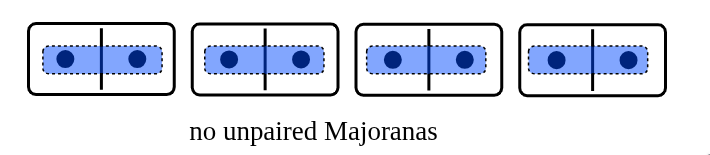
\includegraphics[width=0.45\textwidth]{figs/no_unpaired.png}
  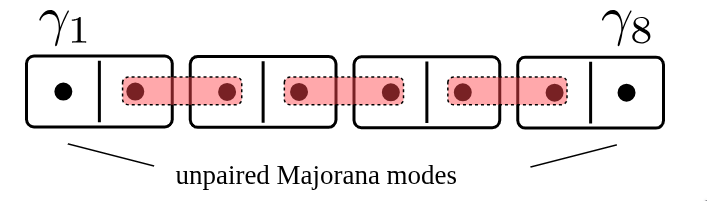
\includegraphics[width=0.45\textwidth]{figs/unpaired.png}
  \caption{Schematic representation of the Kitaev chain in its two distinct phases. Left: In the trivial phase, Majorana modes on the same site pair to form conventional fermions, leaving no unpaired modes. Right: In the topological phase, Majoranas on adjacent sites couple, leaving unpaired modes at the chain ends, which combine into a non-local fermionic mode. \cite{Topocondmat}}
  \label{fig:kitaev}
\end{figure}
In the figure above \ref{fig:kitaev}, we see a schematic representation of the Kitaev chain in its two distinct phases, the trivial phase on the left and the topological phase on the right.\\
In the trivial phase, the Majorana modes on the same site pair to form conventional fermions, leaving no unpaired modes. In contrast, in the topological phase, Majoranas on adjacent sites couple, leaving unpaired modes at the chain ends, which combine into a non-local fermionic mode. At first glance, it may seem impossible to isolate a single Majorana mode, since condensed matter systems are composed of electrons, which always correspond to pairs of Majoranas. However, it turns out that by engineering the Hamiltonian appropriately, one can create a situation where two Majorana modes localize at opposite ends of a one-dimensional system, effectively separating them spatially. This separation is crucial for their non-Abelian statistics and potential applications in topological quantum computing \cite{Topocondmat}.\\
The Hamiltonian of the Kitaev chain is given by:
\begin{equation}
H = -\mu \sum_{j=1}^{N} \left(c_j^\dagger c_j - \frac{1}{2}\right)
- t \sum_{j=1}^{N-1} \left(c_j^\dagger c_{j+1} + c_{j+1}^\dagger c_j\right)
+ \Delta \sum_{j=1}^{N-1} \left(c_j c_{j+1} + c_{j+1}^\dagger c_j^\dagger\right),
\label{eq:kitaev_ham}
\end{equation}
where $μ$ is the chemical potential, or onsite energy, $t$ is the hopping amplitude, and $Δ$ is the p-wave pairing amplitude. The fermionic operators $c_j^\dagger$ and $c_j$ create and annihilate an electron at site $j$, respectively.\\
With the parameters $t=Δ=0$ and $μ ≠ 0$, the system is in a trivial insulating phase with no special edge states. However, tuning the parameters such that $t = Δ > 0$ and $μ = 0$, the edges become isolated, leaving two unpaired Majorana modes localized at the ends. These modes combine into a single non-local fermionic mode that costs zero energy to occupy. We will later explore how this model maps onto the QD–SC–QD system, and how the parameters can be tuned experimentally to reach this regime. 

\paragraph{Bulk Spectrum and Topological phases}
To understand when the Kitaev chain supports topologically non-trivial states, we now turn from the real-space picture to its bulk description in momentum space. This transformation allows us to analyze the quasiparticle excitation spectrum and identify the conditions under which the superconducting gap closes and reopens.\\
Using translation invariance, we apply a Fourier transform,
$$
c_j = \frac{1}{\sqrt{N}} \sum_p e^{ipaj} c_p,
$$
This allows us to write the Hamiltonian (\ref{eq:kitaev_ham}) in momentum space $p$ as:
\begin{equation}
H = ∑_{ p}^{} ξ_p\left(c_p^{†} c_p - \frac{1}{2}\right) - ∑_{p}^{} t \cos p a + Δ ∑_{p}^{}\left(c_p^{†} c_{-p}^{†} e^{ipa} + c_{-p} c_p e^{-ipa}\right), 
\end{equation}
with $ξ_p = -μ - 2t \cos pa$ and $a$ the lattice spacing. This Hamiltonian becomes diagonal in the Bogoliubov–de Gennes (BdG) formalism. The resulting quasiparticle energy spectrum is:
\begin{equation}
  E_{p,\pm} = \pm \sqrt{(μ + 2t \cos{pa})^2 + 4Δ^2 \sin^2{pa}},
\end{equation}
The spectrum is gapped for most parameter values, but the gap closes when
$$
|μ| = 2|t|
$$
See Figure ~\ref{fig:kitaev_bands} for a visualization of the quasiparticle energy spectrum. This marks the critical point separating two distinct superconducting phases. When $μ$ crosses this boundry, the system undergoes a topological phase transition: the character of the ground state changes without any symmetry breaking, but through a change in the topology of the quasiparticle band structure \cite{Qtech}.\\
\begin{figure}
  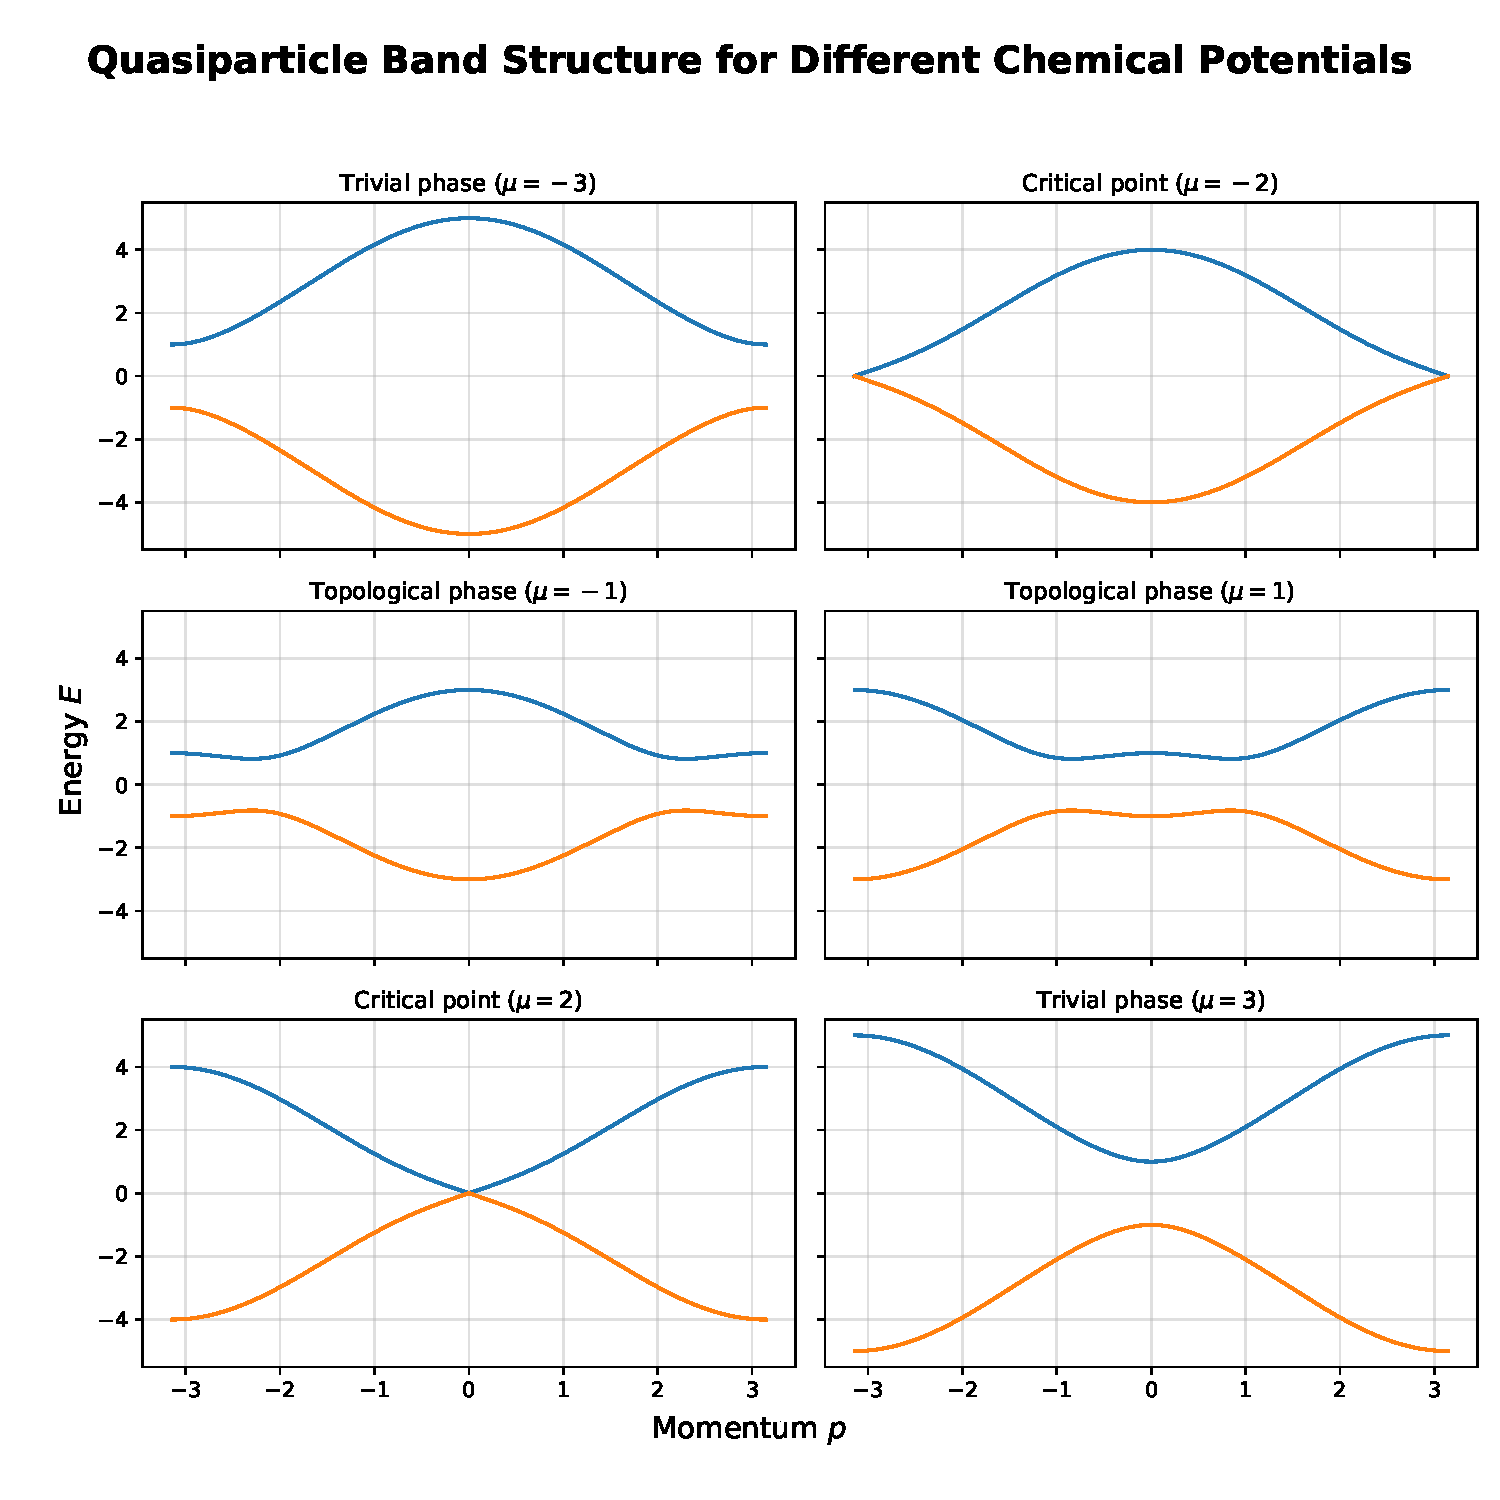
\includegraphics[width=1\textwidth]{figs/band_structure.pdf}
  \caption{Quasiparticle energy spectrum of the Kitaev chain for different chemical potentials $μ$. Left: In the trivial phase ($|μ| > 2|t|$), the spectrum is fully gapped with no zero-energy modes. Right: In the topological phase ($|μ| < 2|t|$), the gap closes and reopens, signaling the emergence of zero-energy edge modes.}
  \label{fig:kitaev_bands}
\end{figure}
% \newpage
\paragraph{Majorana Representation and Zero Modes}
In order to further understand the nature of these boundry states, we can express each fermionic operator in terms of two real Majorana operators:
\begin{equation}
c_j = \frac{1}{2}(\gamma_j^A + i\gamma_j^B), \quad
c_j^\dagger = \frac{1}{2}(\gamma_j^A - i\gamma_j^B),
\label{eq:first_majorana_rep}
\end{equation}
where $\gamma_j^{A,B}$ satisfy $\{\gamma_j^\alpha, \gamma_k^\beta\} = 2\delta_{jk}\delta_{\alpha\beta}$ and $(\gamma_j^\alpha)^\dagger = \gamma_j^\alpha$.\\
In this basis, the two distinct phases correspond to different pairing patterns between the Majorana operators. For a large $μ$, ($|μ| > 2|t|$), the Majorana operators pair up on the same site, leading to a trivial phase with no zero-energy modes. On the other hand, in the topological phase ($|μ| < 2|t|$) and $t = Δ$, the Majoranas on adjacent sites couple ($\gamma_j^B$ with $\gamma_{j+1}^A$), leaving two unpaired Majorana modes at the ends of the chain: $\gamma_1^A$ at the left end and $\gamma_N^B$ at the right end, see Figure \ref{fig:kitaev}.\\
These two unpaired Majoranas combine into a single non-local fermionic mode:
\begin{equation}
  f = \frac{1}{2 }(\gamma_1^A + i\gamma_N^B),
\end{equation}
which satisfies $\{f, f^\dagger\} = 1$ and costs zero energy. The two possible occupations of this non-local fermion correspond to a twofold degenerate ground state. This degeneracy is topologically protected: local perturbations cannot lift it unless they close the bulk gap or couple the two edge Majoranas directly.\\
The Kitaev chain thus provides the minimal theoretical framework for understanding Majorana zero modes. Its simplicity allows for exact solutions and clear physical intuition, making it an ideal starting point for exploring more complex systems that can host topological superconductivity and Majorana fermions.

\subsubsection{The QD-SC-QD System as an Effective Kitaev Chain}
While the Kitaev chain provides the minimal theoretical framework for understanding Majorana zero modes, it remains an abstract model, assuming spinless fermions and idealized $p$-wave pairing. Real materials, however, are spinful and typically host conventional $s$-wave superconductivity. The challenge, therefore, is to engineer hybrid systems whose effective low-energy behaviour mimics that of the Kitaev chain.\\
A particularly compact realization of such a system is the double quantum dot coupled via a superconducting segment, the so-called \textit{Poor Man’s Majorana} (PMM) setup. This device consists of two quantum dots (QDs) connected through a central superconductor, forming the minimal two-site analogue of the Kitaev chain. Despite its simplicity, it reproduces the essential ingredients of topological superconductivity: coherent hopping, non-local pairing, and the emergence of near-zero-energy states with Majorana-like characteristics.

\paragraph{Mapping to the Kitaev Hamiltonian}

Each quantum dot represents a site in the minimal Kitaev chain. The Hamiltonian of the hybrid system can be written in a general form as:
\begin{equation}
H = \sum_{i=L,R} \epsilon_i n_i
+ t (d_L^\dagger d_R + d_R^\dagger d_L)
+ \Delta (d_L^\dagger d_R^\dagger + d_R d_L)
+ U \sum_{i=L,R} n_i
\label{eq:qdsqdh}
\end{equation}
where $d_{L/R}^\dagger$ and $d_{L/R}$ are electron creation and annihilation operators on the left and right dots. $n_i$ is the number operator for dot $i$. The parameters $ϵ_{L,R}$ correspond to the dot energy levels, $t$ is the elastic cotunneling amplitude, $Δ$ is the crossed Andreev reflection amplitude, and $U$ is the on-site Coulomb repulsion energy.\\
The meaning of each parameter is as follows:
\begin{itemize}
    \item \textbf{Elastic cotunneling (ECT):} An electron tunnels coherently from one dot to the other via a virtual process through the superconductor. This process defines the effective hopping amplitude $t$, analogous to the kinetic term in the Kitaev model.
    \item \textbf{Crossed Andreev reflection (CAR):} A Cooper pair in the superconductor splits such that one electron tunnels into each dot. This process produces an effective non-local pairing term $\Delta$, which is mathematically equivalent to the $p$-wave pairing amplitude in the Kitaev chain.
    \item \textbf{On-site energy:} The local dot energies $\epsilon_L$ and $\epsilon_R$ play the role of the site-dependent chemical potential $\mu$.
\end{itemize}
At the so-called sweet spot, where $|\epsilon_L| = |\epsilon_R| = 0$ and $|t| = |\Delta|$, the system enters a regime in which two Majorana-like states localize predominantly on separate dots. These two states form an effective non-local fermion and exhibit many of the qualitative features of true topological Majorana bound states, such as zero-energy modes and near-perfect particle–hole symmetry. However, since the system is finite and lacks a bulk, it does not possess true topological protection, hence the name “poor man’s Majoranas”. \cite{Qtech}

\paragraph{Low-energy Features and Experimental Tunability}
The poor man's Majorana setup, double quantum dot coupled via a superconductor, provides a minimal realization of the Kitaev chain. In reality, the complete microscopic Hamiltonian includes interactions and spin degrees of freedom. However, in the regime relevant for Poor Man's Majoranas, the low-energy physics is effectively captured by the spinless two-site model introduced above. In this setup, near-zero energy Majorana-like states emerge across the two dots, exhibiting an even- and odd-parity ground state and strong non-local correlations.\\
This platform is an experimentally attractive method to realize Kitaev chain physics because its parameters can be tuned independently. Gate voltages control the dot energy levels, the transparency of the QD–SC interfaces governs the effective hopping and non-local pairing, and magnetic fields can suppress unwanted spinful excitations. By sweeping these parameters, one can access and identify the  Majorana-like properties. \\
This minimal setup captures the essential low-energy properties of a Kitaev chain while remaining experimentally controllable, providing a direct route from theoretical modeling to realizable quantum devices.

\subsubsection{Identifying Majorana Modes in the QD-SC-QD System}
In this section we will briefly go through the key signatures that indicate the presence of Majorana-like modes in the QD–SC–QD system. These signatures arise from the unique properties of Majorana fermions. There are a few quantities we can use to identify the presence of PMMs, and their Robustness to perturbations.\\

\paragraph{The parity Operator}
The parity operator itself is not a measurement of a Majorana mode, but it is a useful tool in the identification process. The mean-field Hamiltonian of a superconductor does not conserve particle number, but it does conserve fermion parity. What this means is that the number of electrons in the system can change by pairs, but not by single electrons. The parity operator is defined as:
$$
P = (-1)^{N} = Π_n(1 - 2c_n ^{†} c_n)
$$
where $N$ is the total number of electrons in the system, and $c_n^{†}$ and $c_n$ are the creation and annihilation operators for the fermionic mode formed by the two Majorana modes. The eigenvalues of the parity operator are $+1$ for even parity (an even number of electrons) and $-1$ for odd parity (an odd number of electrons).\\
When working with Majorana modes, we often consider the two degenerate ground states of the system, which differ by their fermion parity. The presence of a Majorana mode implies that these two states are nearly degenerate and can be transformed into each other by adding or removing a single electron, thus changing the parity.\\

\paragraph{Energy Degeneracy}
When we try to identify Majorana modes in the QD–SC–QD system, one of the primary signatures we look for is the presence of energy degeneracy (Figure ~\ref{fig:gs_symmetry}) between the even and odd parity ground states. We also want the ground state energies to be separated by a finite energy gap from the excited states. This energy gap protects the Majorana modes from local perturbations and thermal excitations, which is crucial for their stability and potential use in quantum computing. This is because when we want to do quantum computation using Majorana modes, we need to be able to manipulate the states without causing transitions to higher energy states.\\
\begin{figure}
  \centering
  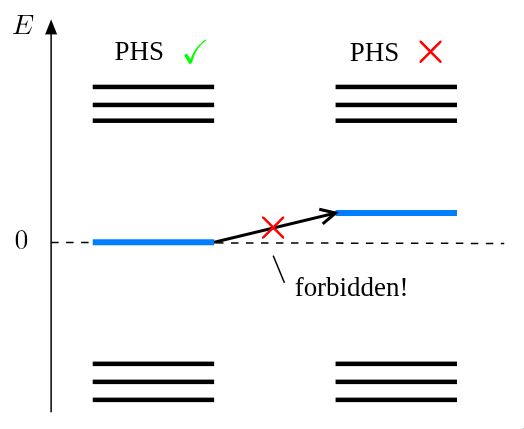
\includegraphics[width=0.5\textwidth]{figs/gs_symmetry}%
  \caption{Energy spectrum showing how the energy eigenvalues of the system must be symmetric around zero energy due to particle-hole symmetry \cite{Topocondmat}.}
  \label{fig:gs_symmetry}
\end{figure}

\paragraph{Local Distinguishability}
A property of the Kitaev chain in its topological phase is that measurements done locally cannot reveal if the system is in its odd or even ground state. Meaning the two ground states are locally indistinguishable. In order to quantify this property, we will define the local distinguishability parameter LD as:
$$
\text{LD} = \frac{1}{N} \sum_{j=1}^{N} || ρ_j^o - ρ_j^e || = \frac{1}{N} \sum_{j=1}^{N} || δ ρ_j ||
$$
\cite{Lund1}, \cite{VikMar}.
Here, $ρ_j^{o/e}$ are the reduced density matrices of site $j$ for the odd and even parity ground states, respectively. The norm $|| \cdot ||$ is the trace norm, which measures the difference between the two local states. The LD parameter quantifies how distinguishable the two ground states are when only local measurements are considered. A value of LD close to zero indicates that the two states are nearly indistinguishable locally, which is a hallmark of Majorana modes. Conversely, a value close to one indicates that the states can be easily distinguished by local measurements, suggesting the absence of Majorana modes.\\

\paragraph{Majorana Polarization}
In interaction Kitaev chains with finite magnetic fields, there are no ideal Majorana sweet spots, as the presence of the other spin species introduces corrections to the simple picture of Majorana modes. However, sweet spots with very good Majorana localization and close to degenerate ground states with even and odd parity can still appear in the system. To quantify how close we are to an ideal Majorana mode, we can use the Majorana polarization (MP) metric. The MP is a measure of how well the Majorana modes are localized at the ends of the chain and how closely they resemble ideal Majorana fermions. The MP is defined as:
$$
M_α = \frac{W_α^2 - Z_α^2}{W_α^2 + Z_α^2}
$$
where,
$$
W_α = ∑_{σ} \bra{o} c_{ασ} + c_{ασ}^{†} \ket{e}, \quad Z_α = i ∑_{σ} \bra{o} c_{ασ} - c_{ασ}^{†} \ket{e}
$$
Here, $α$ denotes the site index (left or right dot), $σ$ is the spin index, and $\ket{o}$ and $\ket{e}$ are the odd and even parity ground states, respectively. In an ideal sweet spot where two Majoranas are perfectly localized on the left and right dots, the MP values would be $M_L = -M_R = ± 1$. \cite{Qtech}.\\

\paragraph{Charge Expectation and non-locality}
The last measurable property we will discuss is the charge expectation value of the ground states. This id measured by taking the expectation values of the number operators in the odd and even ground states:
$$
\bra{e}n_{L(R)} \ket{e}, \quad \bra{o}n_{L(R)} \ket{o}
$$
where $n_{L(R)}$ is the number operator for the left (right) dot. In the ideal case, these expectation values should be equal for both ground states. This is because, if the difference is zero, the two ground states share the same local charge distribution, making them locally indistinguishable. 

\subsection{Braiding of Majoranas}
The process of braiding Majorana modes, in simple terms, involves exchanging the positions of two Majorana modes in a way that their quantum states are transformed.
The reason braiding of Majorana modes is important to discuss is because it is the key operation that allows us to manipulate the quantum information stored in these modes. Braiding refers to the process of exchanging the positions of two Majorana modes in a way that their quantum states are transformed according to non-Abelian statistics. This is a fundamental operation for topological quantum computing, as it enables the implementation of quantum gates that are robust against local perturbations.\\
Braiding in the right patterns, with the right systems, can lead to the implementation of a universal set of quantum gates \ref{fig:quantum_gates}, which is necessary for performing arbitrary quantum computations. The non-local nature of Majorana modes means that the information they encode is protected from local sources of decoherence, making them ideal candidates for fault-tolerant quantum computing.{\color{red} SOURCE}\\ 
\subsubsection{Quantum Gates}
In quantum computing, and specifically the quantum circuit model of computation, a quantum gate is a basic quantum circuit operating on a small number of qubits. Quantum gates are the building blocks of quantum algorithms, analogous to classical logic gates in classical computing. They manipulate the state of qubits through unitary transformations, allowing for the creation of superposition and entanglement, which are essential for quantum computation.\\

\begin{figure}
  \centering
  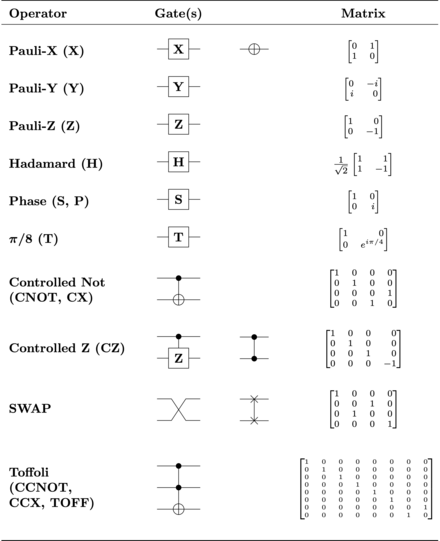
\includegraphics[width = 0.5\textwidth]{figs/Quantum_logic_gates.png}
  \label{fig:quantum_gates}
    \caption{List of common quantum gates and their matrix representations. {\color{red} Wikipedia Quantum logic gates}}
\end{figure}

\paragraph{Pauli gates in terms of fermions}
The gates in focus for this thesis are the Pauli gates, which are represented by the Pauli matrices:

\begin{equation}
X = \begin{pmatrix} 
0 & 1 \\
1 & 0
\end{pmatrix}, \quad
Y = \begin{pmatrix}
0 & -i \\
i & 0
\end{pmatrix}, \quad
Z = \begin{pmatrix}
1 & 0 \\
0 & -1
\end{pmatrix}
\end{equation}
Suppose you have a pair of quantum states $\ket{0}$ and $\ket{1}$, which can be represented as column vectors:
\begin{equation}
\ket{0} = \begin{pmatrix}
1 \\
0
\end{pmatrix}, \quad
\ket{1} = \begin{pmatrix}
0 \\
1
\end{pmatrix}
\end{equation}
Applying the Pauli gates to these states results in the following transformations:
\begin{align*}
X\ket{0} &= \ket{1}, \quad X\ket{1} = \ket{0} \\
Y\ket{0} &= i\ket{1}, \quad Y\ket{1} = -i\ket{0} \\
Z\ket{0} &= \ket{0}, \quad Z\ket{1} = -\ket{1}
\end{align*}
The Pauli-X gate, often reffered to as the NOT gate, flips the state of a qubit. The Pauli-Y gate combines a bit flip with a phase flip, while the Pauli-Z gate applies a phase flip to the $\ket{1}$ state. These gates are fundamental for quantum computation and can be implemented through braiding operations in systems hosting Majorana modes. Other quantum gates can be constructed from these basic gates, and together they form a universal set for quantum computation. The ability to perform these operations through braiding of Majorana modes is what makes them so intriguing for topological quantum computing. \\ 
In order to find out how to implement these gates through baiding, we must first rewrite these gates in terms of simple fermionic operators. 
\begin{align*}
  c_i ^{†} \quad \text{creates a fermion at site } i \\
  c_i \quad \text{annihilates a fermion at site } i
\end{align*}
For a simple two-site system, we can define the fermionic operators for the two sites as $c_1$ and $c_2$. The Pauli gates can be expressed in terms of these operators as follows:

\begin{align*}
  X &= c_1 ^{†} c_2 + c_2 ^{†} c_1 \\
  Y &= -i(c_1 ^{†} c_2 - c_2 ^{†} c_1) \\
  Z &= c_1 ^{†} c_1 - c_2 ^{†} c_2
\end{align*}
which quickly can be verified by applying these operators to the basis states $\ket{0}$ and $\ket{1}$.




\subsubsection{Jordan-Wigner transforms}
The Jordan-Wigner transformation is a transformation that maps spin operators onto fermionic creation and annihilation operators. The reason we want this mapping is that it becomes much easier for us to implement the spin-1/2 Pauli gates in terms of the fermionic operators, which are more natural to implement in our system. We can redefine our fermionic operators in terms of the Pauli matrices as follows:
\begin{align*}
σ_j^+ &= \frac{1}{2}(σ_j^x + iσ_j^y) \equiv f_j ^{†} \\
σ_j^- &= \frac{1}{2}(σ_j^x - iσ_j^y) \equiv f_j \\
σ_j^z &= 2f_j ^{†} f_j - 1
\end{align*}
Now we have the correct same-site fermionic relations $\{f_j ^{†} , f_j\} = I$. However on different sites, we have $\{f_j ^{†} , f_k\} \neq 0$, and $[σ_j^+,σ_k^-] = 0$ for $j \neq k$. So spins on different sites commute, while fermions on different sites anticommute. To fix this, we introduce a string of $σ^z$ operators to ensure the correct anticommutation relations. So we define a new set of fermionic operators as follows:
\begin{equation}
  a_j^{†} = Π_{k=1}^{j-1} (-σ_k^z) ⋅ f_j^{†}, \quad a_j = Π_{k=1}^{j-1} (-σ_k^z) ⋅ f_j
\end{equation}
The transformed spin operators now have the appropriate fermionic canonical anti-commutation relations:
\begin{align*}
\{a_j^{†}, a_k\} &= δ_{jk} \\
\{a_j^{†}, a_k^{†}\} &= 0 \\
\{a_j, a_k\} &= 0
\end{align*}
{\color{red} SOURCE JW WIKIPEDIA}\\ 
\paragraph{Pauli Spin Matrices on Majorana representation}
If we rewrite the majorana representation from equation \ref{eq:first_majorana_rep} in terms of the Jordan-Wigner transformed fermionic operators, we can express the Pauli gates in terms of the Majorana operators. This allows us to see which couplings we need to implement in order to perform the desired quantum gates through braiding of Majorana modes.\\
In order to do so, we can first define four majorana operators, two for each site, in terms of creation and annihilation operators:
\begin{align*}
  c_1 &= (γ_0 + i γ_1)/2 \quad c_1 ^{†} = (γ_0 - i γ_1)/2 \\
  c_2 &= (γ_2 + i γ_3)/2 \quad c_2 ^{†} = (γ_2 - i γ_3)/2
\end{align*}
Then we can express the Pauli gates in terms of these Majorana operators as follows:
\begin{align*}
  X &= c_1^{†} c_2 + c_2^{†} c_1 =  \frac{γ_0 - iγ_1}{2}\frac{γ_2 + iγ_3}{2} + \frac{γ_2 - iγ_3}{2}\frac{γ_0 + iγ_1}{2} \\
    &= \frac{i}{2} (γ_0γ_3 - γ_1γ_2)
\end{align*}
From the odd parity subspace we have the total Parity operator $P_{tot}=i²γ_0γ_1γ_2γ_3=-I$. From this we can try to find a relation between $γ_0γ_3$ and $γ_1γ_2$.
\begin{align*}
  γ_0&γ_1γ_2γ_3 = I\\
  γ_0&γ_1γ_2γ_3 γ_3 = γ_3\\
  γ_0&γ_1γ_2 = γ_3 \\
  γ_1&γ_2γ_0γ_0 = γ_3γ_0\\
  γ_1&γ_2=γ_3γ_0=-γ_0γ_3
\end{align*}

\begin{align*}
  Y &= -i(c_1^{†} c_2 - c_2^{†} c_1) = -i\left(\frac{γ_0 - iγ_1}{2}\frac{γ_2 + iγ_3}{2} - \frac{γ_2 - iγ_3}{2}\frac{γ_0 + iγ_1}{2}\right) \\
    &= -\frac{i}{2} (γ_0γ_2 + γ_1γ_3)
  Y &= -i γ_0γ_2 \text{ or } Y = -i γ_1γ_3
\end{align*}

\begin{align*}
  Z &= c_1^{†} c_1 - c_2^{†} c_2 = \frac{γ_0 - iγ_1}{2}\frac{γ_0 + iγ_1}{2} - \frac{γ_2 - iγ_3}{2}\frac{γ_2 + iγ_3}{2} \\
    &= \frac{i}{2} (γ_0γ_1 + γ_2γ_3)
  Z &= iγ_0γ_1 \text{ or } Z= iγ_2γ_3
\end{align*}
By using the parity conservation and the relation between the Majorana operators, we can express the Pauli gates in terms of different pairs of Majorana operators. So what this means is we can represent the Pauli gates as specific couplings between the Majorana modes:
\begin{align*}
  X &= \frac{i}{2} (γ_0γ_3 - γ_1γ_2) = iγ_0γ_3 = -iγ_1γ_2 \\
  Y &= -\frac{i}{2} (γ_0γ_2 + γ_1γ_3) = -i γ_0γ_2 = -i γ_1γ_3 \\
  Z &= \frac{i}{2} (γ_0γ_1 + γ_2γ_3) = iγ_0γ_1 = iγ_2γ_3
\end{align*}

\paragraph{Majorana Exchange Gates}
We can take a step towards braiding by defining Majorana exchange operators. We need to find unitaries $B_{ij}$ that exchange Majoranas $γ_i$ and $γ_j$ while leaving the others unchanged. Meaning they should act as follows:
\begin{align*}
B_{ij} γ_i B_{ij} ^{†} &= γ_j \\
B_{ij} γ_j B_{ij} ^{†} &= -γ_i \\
B_{ij} γ_k B_{ij} ^{†} &= γ_k \quad \text{for } k \neq i,j
\end{align*}
So we need to express these unitary gates in terms of the Majorana operators, in a way that relates them to the Pauli gates we want to implement. It turns out that the Majorana exchange operators can be expressed as:
\begin{equation}
B_{ij} = \frac{i}{\sqrt{2}} (1 - γ_i γ_j) \quad B_{ij} ^{†} = \frac{1-i}{\sqrt{2}} (1 + γ_i γ_j)
\end{equation}
Using the combinations of Majorana operators we just found for the Pauli gates, we can express the Majorana exchange operators in terms of the Pauli gates as follows:
\begin{align*}
B_{12}^2 &= -iγ_1γ_2 = -X \\
B_{03}^2 &= iγ_0γ_3 = X \\
B_{02}^2 &= iγ_0γ_2 = -Y\\
B_{13}^2 &= iγ_1γ_3 = -Y\\
B_{01}^2 &= iγ_0γ_1 =  Z\\
B_{23}^2 &= iγ_2γ_3 =  -Z
\end{align*}

\subsubsection{Kato Berry Phase}
Berry phase is a geometric phase acquired by the wavefunction of a quantum system when it undergoes adiabatic evolution around a closed loop in parameter space. In the context of Majorana modes, the Berry phase can be used to characterize the topological properties of the system and to understand how the quantum states transform under braiding operations.\\
In this thesis, the berry phase will help us measure wether or not we manage to implement the desired quantum gates through braiding of Majorana modes. By calculating the Berry phase associated with the braiding process, we can determine if the resulting transformation corresponds to the expected unitary operation on the qubit space defined by the Majorana modes.\\

If we follow a non-degenerate eigenstate of a Hamiltonian as we slowly (adiabatically) change a
parameter in a loop in parameter space, we will end up with the same state up to a phase. The phase
has two contributions, one is dynamical and depends on the actual time scale of the evolution and
the energy of the state. But there is another contribution that is independent of the details of the
evolution. It only depends on the path taken. It is a geometric quantity and comes from a sort of
curvature in the space of eigenstates. It is called the Berry phase and can be calculated from the
Berry connection $A=i\braket{dψ|ψ}$ integrated during the evolution.
If the state is degenerate, we can get more than a phase. Even for adiabatic evolution, the degenerate
states will mix together. Thus, the Berry phase will be represented by a matrix that mixes the states
together. The Berry connection is also a matrix with a dimension equal to the number of degenerate
states: $A_{nm} = i \braket{dψ_n|ψ_m}$. 

A nice way to calculate non-abelian Berry phase is known as the Kato method. This method uses the projector $P$ that projects on the two degenerate ground
states. Then one solves the differential equation
$$
∂_{t}U_t = i \left[P, ∂_{t}P\right]U_t \\
U_0 = I
$$
and the final unitary is the non-abelian Berry phase $U_{T}$. It shouldn’t matter if the total time $T$ is long or short. $UT$ is the gate that a proper adiabatic evolution would implement. Note that the projector $P$ is time-dependent. It can be calculated numerrically by diagonalizing the Hamiltonian, or analytically if the hamitonian is simple enough. 


\subsubsection{Effective Braiding Hamiltonian}
If we assume that we already have a system with four Majorana modes, we are able to write down an effective Hamiltonian that describes the couplings between these Majorana modes. 
\begin{figure}
  \centering
  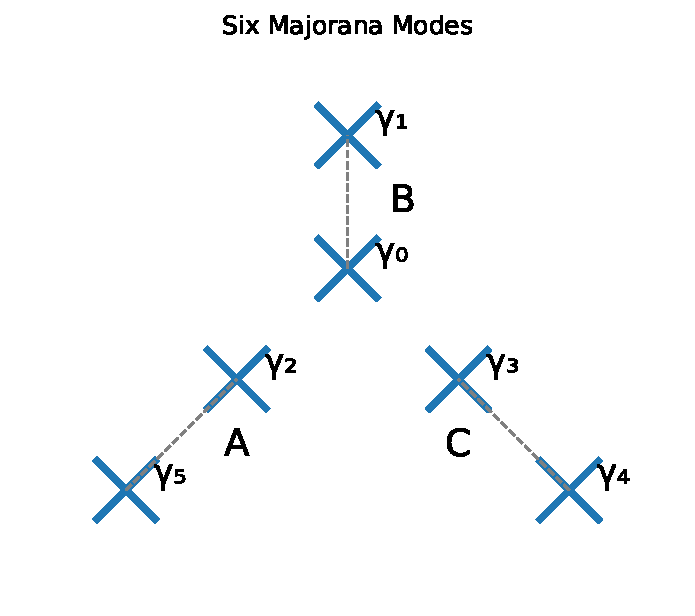
\includegraphics[width=0.5\textwidth]{figs/sixmajoranas.pdf}
  \caption{Schematic representation of a system hosting six majoranas. The illustrations shows pairs of two and two Majoranas coupling together, in a Y-junction, each pair form a subsystem that can be described by a Poor Man’s Majorana setup, A, B and C.}
  \label{fig:6_majoranas}
\end{figure}
In the figure above \ref{fig:6_majoranas}, we see a schematic representation of a system hosting six Majorana modes, arranged in a Y-junction. The Majorana modes are represented by the X-markers. In the figure we see that the Majoranas are coupled in pairs. This represents a standard initial state of three Poor Man’s Majorana setups, where each pair represents the emerging edge modes of each setup. \\
The four most relevant Majorana modes for our braiding operation are the ones labeled as $γ_0$, $γ_1$, $γ_2$, and $γ_3$. While the other two Majoranas, $γ_4$ and $γ_5$, are coupled together and form a non-local fermionic mode that is not involved in the braiding process. The effective Hamiltonian describing the couplings between the four Majorana modes can take the simple form of:
\begin{equation}
  \begin{aligned}
    H = &Δ_{01} iγ_0γ_1 + \\
    &Δ_{02} iγ_0γ_2 + \\
    &Δ_{03} iγ_0γ_3 
  \end{aligned}
  \label{eq:H_eff}
\end{equation}
where $Δ_{ij}$ represents a tunable coupling strength between Majorana modes $γ_i$ and $γ_j$. In reality this $Δ_{ij}$ will be a function of the physical parameters of the system, such as the tunneling amplitudes, the superconducting gap, and the gate voltages. By tuning these parameters to the correct values, we can control the couplings between the Majorana modes and thus implement the desired braiding operations.\\ \\
The $Δ$ in the effective Hamiltonian is a simplified version of what we would have in a real system. In a more realistic model, we would replace these, with a intra PMM junction coupling. However, if we look back at our Poor Mans Hamiltonian \ref{eq:qdsqdh}, the recipe for the junction Hamiltonian are the same coupling effects as the effective Hamiltonian. In essence, we are just extending a Poor Man’s Majorana to where if a coupling is turned on, we just have one longer PMM chain, and one shorter. So if we want to couple $γ_0$ and $γ_2$, we would now have a chain connecting $γ_0, γ_1, γ_2, γ_5$. Where the coupling now can be represented by turning on a new superconducting segment between the two PMM setups. This junction Hamiltonian would simply be:
\begin{equation}
  H_{JuncAB} = t_{AB} (d_{A} ^{†} d_{B} + d_{B} ^{†} d_{A}) + Δ_{AB} (d_{A} ^{†} d_{B} ^{†} + d_{B} d_{A})
  \label{eq:junctionHamiltonian}
\end{equation}
but if we are simply testing out if our braiding protocol works, and we have stable Majorana modes, we can just use the effective Hamiltonian in equation \ref{eq:H_eff} to simulate the braiding process and calculate the resulting Berry phase. This allows us to verify if the braiding operation implements the desired quantum gate on the qubit space defined by the Majorana modes.

\subsection{Sweet spot parameter search}
The Poor Man’s Majorana setup is a highly tunable system, with several parameters that can be adjusted to access different regimes of the system. We know of certain non-interacting sweet spots where the Majorana modes are perfectly localized and the ground states are exactly degenerate. However, in the presence of interactions, these ideal sweet spots may no longer exist. \\
In an ideal system, we would have a perfect sweet spot where the Majorana modes are perfectly localized on the left and right dots and with degeneracy protection accross multiple energy levels, for topological protection. \\ \\
As we found in \ref{KitaevChains}, we very well know the ideal parameters for a non-interacting two-dot system. However, when introducing interactions, the parameter space becomes slightly more complex. And it does not seem possible to find degeneracy accross multiple energy levels, which is preferable for topological protection. However, there is no evidence that it is not possible to find such a sweet spot if you increase the number of quantum dots in the system, creating longer chain. Figure \ref{fig:PMM_setup} shows a schematic representation of a three-dot system, where we can see that there are multiple tunable parameters. The more dots we add, the more tunable parameters we have. But with more tunable parameters, the problem of finding a sweet spot analytically becomes very complex, especially if we dont rely on symmetries and assumptions. Therefore, we will need to explore the parameter space numerically, using optimization techniques to find the sweet spots where Majorana-like modes emerge.\\
\begin{figure}
  \centering
  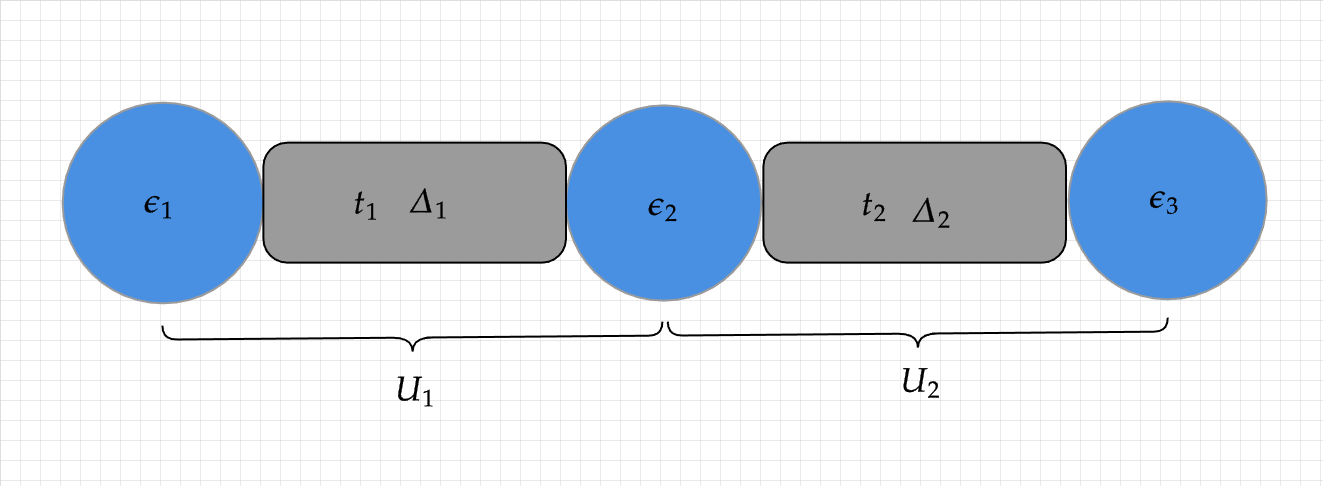
\includegraphics[width=0.8\textwidth]{figs/PMMSetup.png}
  \caption{Schematic representation of the PMM setup. The three quantum dots are represented by the blue circles, and the superconducting segments are represented by the grey rectangles. The tunable parameters of the system, such as the dot energy levels, ECT, CAR and the coloumb interaction, are indicated by their respective labels. By tuning these parameters, we can access different regimes of the system and identify the sweet spots where Majorana-like modes emerge.}
  \label{fig:PMM_setup}
\end{figure}
\subsubsection{General Loss function}\label{Lossfunctionsection}
For a simple two-dot system, we have a total of 5 tunable parameters: the dot energy levels $\epsilon_L$ and $\epsilon_R$, the elastic cotunneling amplitude $t$, the crossed Andreev reflection amplitude $Δ$, and the on-site Coulomb repulsion energy $U$. If we introduce a third dot, we get 9 independent tunable parameters, assuming the interaction strengths can be different for each dot. With more dots, the number of tunable parameters increases significantly, making the parameter space more complex and harder to explore analytically, vizualised in \ref{fig:paramVisualization}.\\
Before setting up the optimization problem, we need to define a loss function that quantifies how close we are to finding a sweet spot with Majorana-like modes. This loss function should take into account the key signatures of Majorana modes, such as energy degeneracy and gap, local indistinguishability, Majorana polarization, and charge expectation values. By minimizing this loss function, we can identify the regions in parameter space where Majorana-like modes are likely to emerge.\\
The loss function can be defined as a weighted sum of the different metrics that characterize the presence of Majorana modes. The weights can vary depending on the importance we assign to each metric. For example ground state degeneracy and gap is much more important than the gap and degeneracy of the higher energy levels, so we can assign a higher weight to the first one, gradiually decreasing the weights for the higher energy levels. Other metrics, defining for Majoranas, such as local indistinguishability, charge expectation values, and Majorana polarization should be included with a significant weight, as they are crucial for the identification of Majorana modes.
\subsubsection{Gradient Descent and Basin-Hopping}
Once we have defined our loss function, we can use optimization techniques to explore the parameter space and find the sweet spots. Gradient descent is a common optimization algorithm that iteratively updates the parameters in the direction of the negative gradient of the loss function. However, due to the complex landscape of the parameter space, with multiple local minima, gradient descent may get stuck in a local minimum and fail to find the global minimum corresponding to the ideal sweet spot.\\ \\
If a multi-variable function, such as our loss function $L(Θ)$, is defined and differentiable in a neighborhood of a point $Θ_0$, then $L(Θ)$ decreases fastest if one goes from $Θ_0$ in the direction of the negative gradient of $L$ at $Θ_0$, denoted as $-∇L(Θ_0)$. If:
$$
Θ_{n+1} = Θ_n - α ∇L(Θ_n)
$$ {\color{red} WIKI Gradient descent}for some positive scalar $α$, then $L(Θ_{n+1}) < L(Θ_n)$, at least for sufficiently small $α$. The parameter $α$ is called the learning rate. Iteratively, this method will converge to a local minimum of the loss function. However, our parameter space is likely to have multiple local minima.\\
In order to overcome this issue, we can use a more sophisticated optimization technique called basin-hopping. Basin-hopping is a global optimization technique that iteratively performs local optimization (such as gradient descent) followed by a random perturbation of the parameters. \\
The algorithm works as follows:
\begin{itemize}
  \item Start with an initial guess for the parameters $Θ_0$.
  \item Perform a local optimization (e.g., gradient descent) to find a local minimum of the loss function, resulting in parameters $Θ_{local}$.
  \item Randomly perturb the parameters to escape the local minimum, resulting in new parameters $Θ_{new}$.
  \item Perform another local optimization starting from $Θ_{new}$ to find a new local minimum, resulting in parameters $Θ_{new\_local}$.
  \item If the loss function at $Θ_{new\_local}$ is lower than the loss function at $Θ_{local}$, accept $Θ_{new\_local}$ as the new current solution; otherwise, keep $Θ_{local}$.
  \item Repeat for a suiting number of iterations or until convergence criteria are met.
\end{itemize}
Basin-hopping allows us to explore the parameter space more effectively and increases the chances of finding the global minimum corresponding to the ideal sweet spot with Majorana-like modes. By combining local optimization with random perturbations, we can navigate through the complex landscape of the loss function and identify the optimal parameters for realizing Majorana modes in our system. \\ \\
However, it is important to note that this optimization process, as any optimization process, will return the best parameter solution it can find. It is not a given that it will find a set of parameters that corresponds to a perfect sweet spot with ideal Majorana modes, but it can still find an approximate sweet spot, which can point us in the right direction and give us insights into the parameter regimes where Majorana-like modes are likely to emerge.  


\begin{figure}
\centering
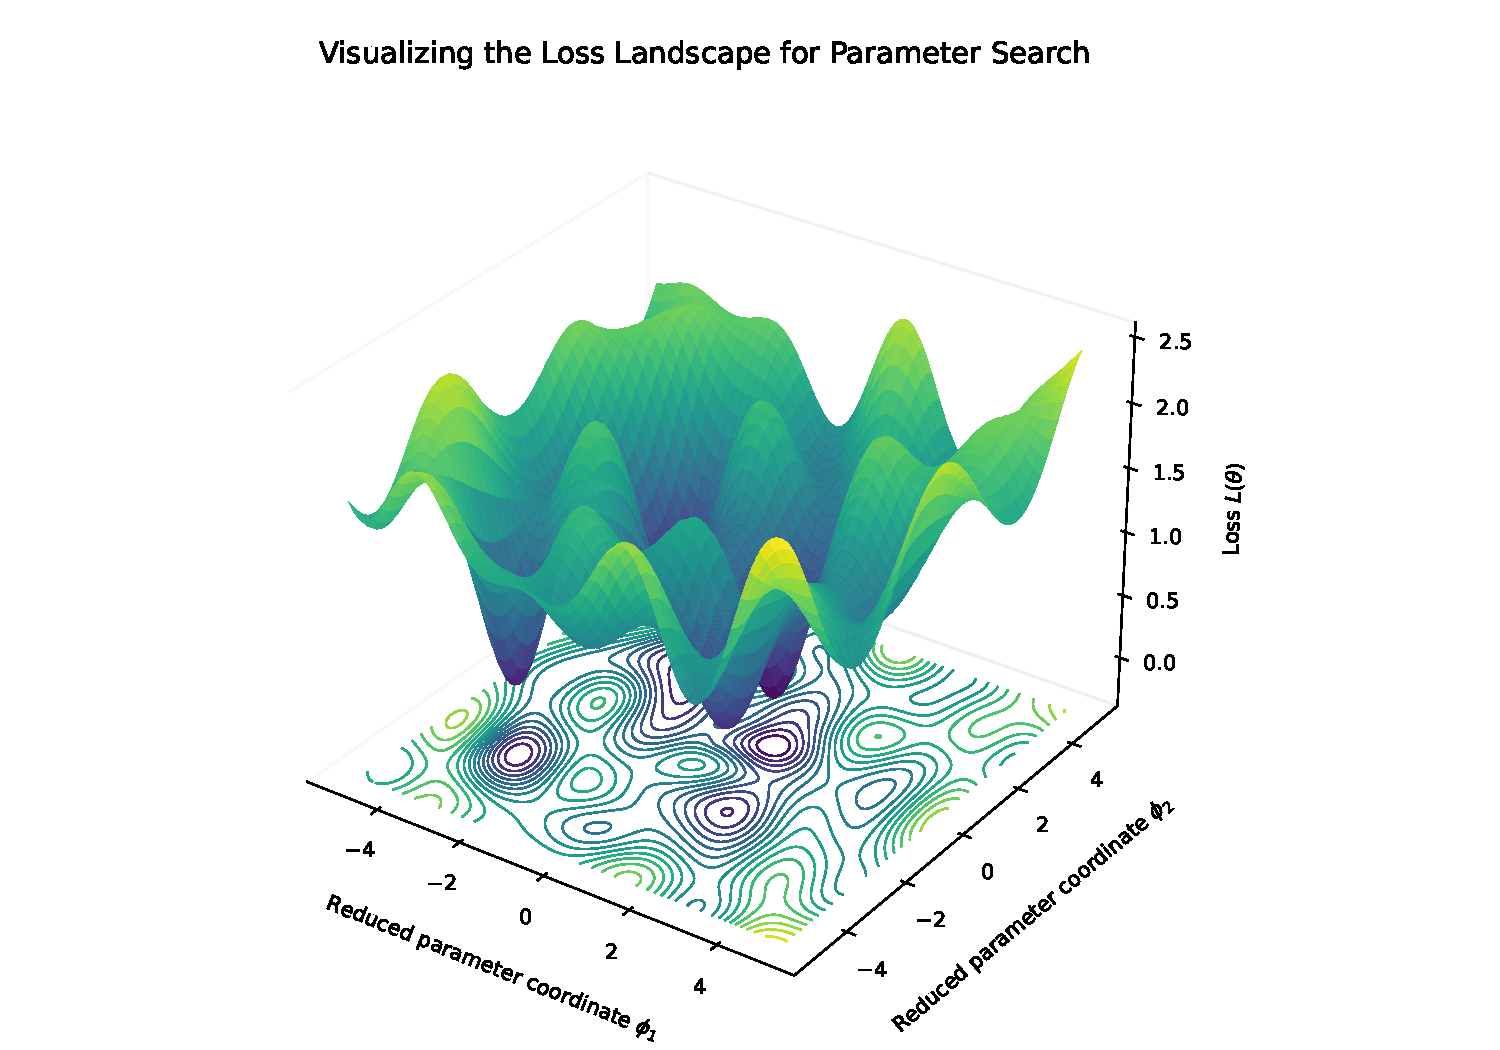
\includegraphics[width=\textwidth]{figs/3dparametersearch.pdf}
\caption{Visualization of the parameter space for an n-dot system, showing how multiple parameters and their combinations create a complex landscape with multiple local minima.}
\label{fig:paramVisualization}
\end{figure}
